% CouncilHound: how it works --- technical white paper
% Build: tectonic docs/councilhound-white-paper.tex
\documentclass[11pt]{article}

\usepackage[margin=1.1in]{geometry}
\usepackage{amsmath, amssymb}
\usepackage{booktabs}
\usepackage{array}
\usepackage{tabularx}
\usepackage{microtype}
\usepackage[hidelinks]{hyperref}
\usepackage{enumitem}
\usepackage{xcolor}
\usepackage{tikz}
\usetikzlibrary{arrows.meta, positioning, fit, backgrounds, calc}
\setlist{itemsep=2pt, topsep=4pt}

\definecolor{pine}{HTML}{1F4D3A}
\definecolor{cream}{HTML}{FFFAF0}

\newcommand{\code}[1]{\texttt{#1}}
\newcolumntype{L}{>{\raggedright\arraybackslash}X}

\title{CouncilHound: Turning a City's Meeting Record into a Searchable, Askable Knowledge Base}
\author{Hunter Brown \\ \small\href{mailto:huntermbrown@gmail.com}{\texttt{huntermbrown@gmail.com}} \\ \small\href{https://councilhound.net}{\texttt{councilhound.net}}}
\date{October 2026 \\ \small describes the system as deployed from \code{main} (City of Fairfax, Virginia)}

\begin{document}
\maketitle

\begin{abstract}
\noindent
Local government decisions are made in public, but the public record is hard to use:
hours of unindexed video, agendas and minutes scattered across PDF viewers, and project
histories that span years of meetings and several boards. CouncilHound is an open
pipeline and web application that reads a city's Granicus meeting archive and its
development-project records every night and turns them into a structured knowledge base
of meetings, agenda items, roll-call votes, tracked projects and topics, members' voting
records, speaker-attributed transcripts, and project wikis. Residents can browse it,
search it, follow it by email, or ask it questions in plain language, and every claim
leads back to the source document or the exact second of the city's own video.
Ahead of a city election it also publishes a ballot guide that treats every candidate
alike, drawing on dated, hand-verified outside sources.
This paper describes what data CouncilHound collects, how each stage of the pipeline
processes it, where language models are used and how their output is constrained,
and how the results are served. A companion report,
\emph{CouncilHound Development Impact Methodology}, documents the economic and fiscal
impact models separately.
\end{abstract}

\tableofcontents
\newpage

%=====================================================================
\section{Motivation and scope}

A typical small-city council meets twice a month for three hours or more. Its planning
commission, school board, and advisory boards add more meetings. A resident who wants to
know ``what happened with the townhomes on Park Road'' has to know which meetings to
open, scrub through the recordings, and read packets that can run to hundreds of pages.
Professional observers (reporters, neighborhood associations, members themselves) face
the same problem at a larger scale.

CouncilHound answers four questions from the record:
\begin{enumerate}
  \item \textbf{What was decided?} Meeting-level ledgers of motions and roll-call votes,
        with procedural items filtered out.
  \item \textbf{Where does a matter stand?} A history and current status for every
        project, ordinance, case, and recurring topic, assembled across meetings and bodies.
  \item \textbf{Who voted how, and who said what?} Per-member voting records, pairwise
        agreement, and speaker-attributed transcript passages.
  \item \textbf{What is coming up?} Upcoming agendas annotated with the tracked matters
        they name and whether a public hearing is scheduled.
\end{enumerate}

The reference deployment tracks the City of Fairfax, Virginia: its City Council,
Planning Commission, School Board, Parks and Recreation Advisory Board (PRAB), and
Housing and Healthy Communities Advisory Board (HHCAB). The pipeline is written against
the Granicus platform, which hosts meeting archives for hundreds of U.S.\ local
governments, so it can be pointed at another Granicus city with configuration changes
(Section~\ref{sec:portability}).

%=====================================================================
\section{Design principles}
\label{sec:principles}

Five rules shape the system. Most of the implementation choices described later follow from them.

\begin{enumerate}
\item \textbf{The city's record is the source of truth.} CouncilHound derives everything
      from public documents and recordings, and every derived fact keeps a pointer back to
      them: a document URL, a meeting, an agenda-item label, or a timestamp.
\item \textbf{Video is linked, never hosted.} Every ``watch'' affordance is a deep link
      into the city's own Granicus player, seeked to the relevant second. CouncilHound
      never re-hosts, embeds, or proxies meeting video.
\item \textbf{Language models never own identity.} Models extract \emph{names}, and code
      decides which entity a name refers to, when two entities are the same, and who a
      speaker is allowed to be named as. A model's output can never create or merge a
      record's identity on its own.
\item \textbf{Constrain, verify, and record model output.} Wherever a model is used, its
      output is shaped by a forced tool schema, checked in code against the source text,
      and stored raw with a prompt version so it can be re-applied or audited without
      another call.
\item \textbf{Every stage is idempotent.} Each pipeline stage can be re-run at any time
      and converges on the same state. That makes nightly re-processing, backfills, and
      recovery from partial failure routine operations rather than incidents.
\end{enumerate}

%=====================================================================
\section{System overview}

\begin{figure}[h]
\centering
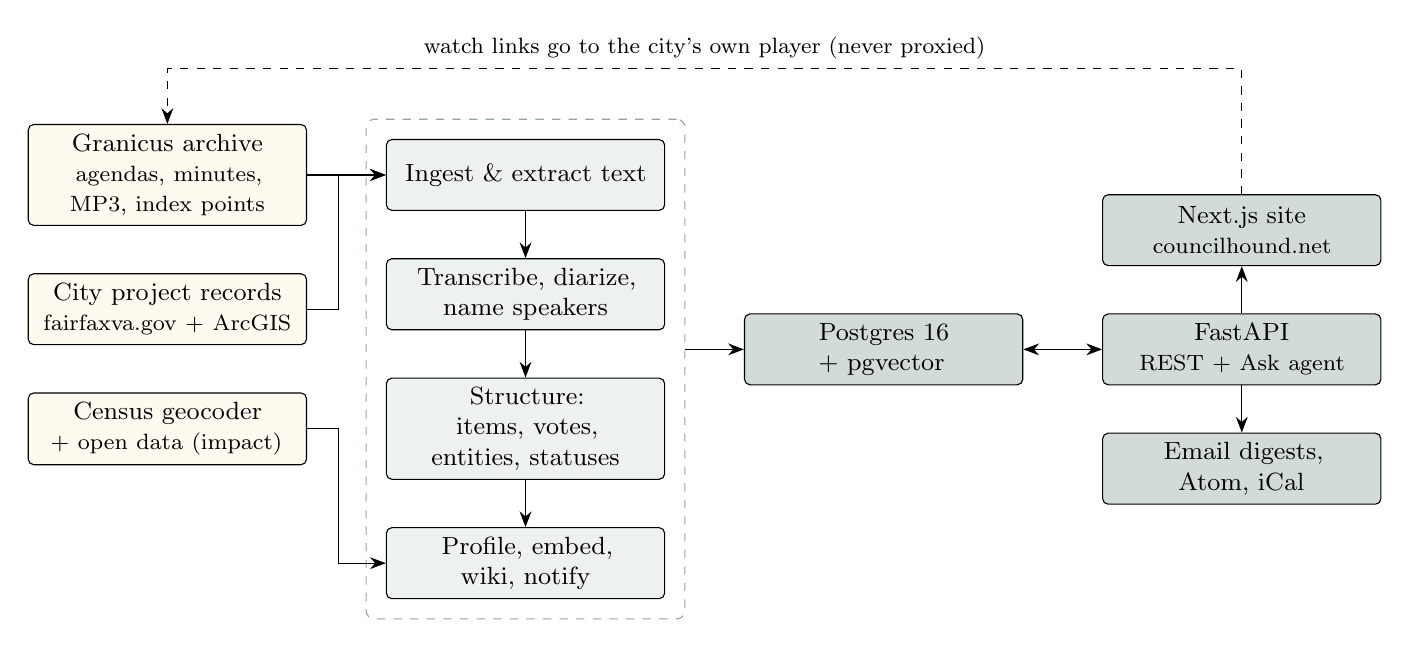
\begin{tikzpicture}[
  node distance=6mm and 10mm,
  box/.style={draw, rounded corners=2pt, align=center, font=\small, minimum height=9mm, text width=33mm, fill=white},
  src/.style={box, fill=cream},
  stage/.style={box, fill=pine!8},
  srv/.style={box, fill=pine!20},
  >={Stealth[length=2mm]}
]
\node[src] (gran) {Granicus archive\\\footnotesize agendas, minutes, MP3, index points};
\node[src, below=of gran] (proj) {City project records\\\footnotesize fairfaxva.gov + ArcGIS};
\node[src, below=of proj] (census) {Census geocoder\\\footnotesize + open data (impact)};

\node[stage, right=of gran] (ing) {Ingest \& extract text};
\node[stage, below=of ing] (tr) {Transcribe, diarize,\\name speakers};
\node[stage, below=of tr] (st) {Structure: items, votes,\\entities, statuses};
\node[stage, below=of st] (en) {Profile, embed,\\wiki, notify};

\node[srv, right=of tr, yshift=-7mm] (db) {Postgres 16\\+ pgvector};
\node[srv, right=of db] (api) {FastAPI\\\footnotesize REST + Ask agent};
\node[srv, above=of api] (web) {Next.js site\\\footnotesize councilhound.net};
\node[srv, below=of api] (mail) {Email digests,\\Atom, iCal};

\draw[->] (gran) -- (ing);
\draw[->] (proj.east) -- ++(4mm,0) |- (ing.west);
\draw[->] (census.east) -- ++(4mm,0) |- (en.west);
\draw[->] (ing) -- (tr);
\draw[->] (tr) -- (st);
\draw[->] (st) -- (en);
\begin{scope}[on background layer]
\node[draw=pine!50, dashed, rounded corners=3pt, inner sep=2.5mm, fit=(ing)(en)] (pipe) {};
\end{scope}
\draw[->] (pipe.east |- db.west) -- (db.west);
\draw[<->] (db) -- (api);
\draw[->] (api) -- (web);
\draw[->] (api) -- (mail);
\coordinate (top) at ($(gran.north)+(0,7mm)$);
\draw[->, dashed] (web.north) -- (web.north |- top) -- node[above, font=\footnotesize]{watch links go to the city's own player (never proxied)} (gran.north |- top) -- (gran.north);
\end{tikzpicture}
\caption{Data flow. Ingestion stages (green, in the dashed box) run as a scheduled batch job; the API and
web front end are read-mostly services over the same database.}
\label{fig:overview}
\end{figure}

CouncilHound has three parts (Figure~\ref{fig:overview}):
\begin{itemize}
  \item an \textbf{ingestion pipeline} (Python 3.12, SQLAlchemy~2, Alembic) exposed as a
        command-line tool whose \code{daily} command chains every stage;
  \item a \textbf{PostgreSQL~16} database with the \code{pgvector} extension, holding both
        relational records and vector embeddings;
  \item a \textbf{FastAPI} service and a \textbf{Next.js~14} front end that serve the
        public site, the plain-language question-answering agent, and the feeds.
\end{itemize}
Production runs on Fly.io (Section~\ref{sec:ops}).

%=====================================================================
\section{Data sources}
\label{sec:sources}

\subsection{Granicus meeting archive}

Granicus is the meeting-video platform behind most U.S.\ municipal ``watch meetings
online'' pages. CouncilHound reads it as an anonymous web visitor would. Every request
carries a browser user agent (Granicus refuses bare clients), is spaced at least one
second apart, and is retried with back-off on server errors and throttling.

\begin{table}[h]
\centering\small
\begin{tabularx}{\linewidth}{@{}lL@{}}
\toprule
Endpoint & What CouncilHound takes from it \\
\midrule
\code{ViewPublisher.php} & The archive listing: one row per recorded meeting with date,
  duration, clip identifier, agenda and minutes links, MP3/MP4 links, and a document
  drop-down (actions reports, minutes, other). The same page carries the
  \emph{upcoming events} table. \\
\code{AgendaViewer.php} & The agenda, either HTML or an uploaded PDF or Word file; through
  \code{GeneratedAgendaViewer}, links to per-item attachments. \\
\code{MetaViewer.php} & Per-agenda-item attachments: staff reports, draft motions,
  resolutions, plans. \\
\code{MinutesViewer.php} & Minutes and the clerk's actions report, which are the
  authoritative record of motions and votes. \\
\code{MediaPlayer.php} & The clerk's \emph{index points}: per-agenda-item timestamps
  in the recording. \\
\code{archive-video.granicus.com} & Meeting audio (MP3) for transcription. \\
\bottomrule
\end{tabularx}
\caption{Granicus endpoints used.}
\end{table}

Granicus serves caption files for these meetings, but they are empty, so CouncilHound
transcribes the audio itself (Section~\ref{sec:transcription}). Granicus's content
network also blocks requests from data-center IP ranges for media files. Audio is
therefore downloaded and transcribed on a residential machine, while everything else
runs in the cloud.

Each archive section is mapped to a tracked \emph{body}. Within a body, a meeting's
title sets its type (regular, work session, special, retreat, closed session). Rows with
no recording, such as cancelled or future meetings, are skipped, and cancelled-meeting
clips are never transcribed because their title-card music makes speech recognition
hallucinate. The two advisory boards publish agendas and minutes but no recordings.

\subsection{Official development-project records}

The city publishes a directory of major development and capital projects. CouncilHound
reads it from two places:
\begin{itemize}
  \item the \textbf{city website's project pages}, which give project type, division,
        official schedule and status, timeline, background, the applicant's requests,
        linked documents, address and coordinates, assigned planner, and project image;
  \item the city's \textbf{ArcGIS feature service} for the major-developments map,
        which gives name, description, applicant, development status (pre-application,
        under review, approved, under construction), project URL, and point geometry.
\end{itemize}
The city website also blocks data-center IPs, so cloud runs fall back to the ArcGIS
layer alone. A partial run never overwrites richer fields gathered earlier and never
deletes a record. Each official project becomes a \code{project} entity, and the meetings
that discuss it are linked to it through the same entity-resolution path used for
meeting-derived topics (Section~\ref{sec:entities}). The site currently carries 41
official project records.

\subsection{Geocoding and open data}

Locations named in meetings (streets, addresses, sites) are geocoded with the U.S.\ Census
Bureau's public geocoder, constrained to the city. Failures are recorded so they are not
retried every night. The development-impact subsystem draws on further open datasets:
American Community Survey block groups, TIGER geography, LEHD origin--destination
employment data, OpenStreetMap street networks, merged Overture, Foursquare, and
OpenStreetMap points of interest, transit GTFS feeds, city GIS layers, and parcel
assessment records (owner names are never stored). Those sources and models are covered
in the companion methodology report.

\subsection{Election and term data}
\label{sec:election-data}

Member terms, seat expirations, and the current ballot (candidates by seat) are pinned
by hand from the city's and registrar's published sources. Each entry records its source
URL and the date it was verified. The data powers term and ballot answers in the
question-answering agent, and an election date stops being reported once it has passed.

\paragraph{Candidates.} Most candidates have never voted at a meeting the record covers,
so the record alone can say nothing about them. A hand-curated table holds, for every
name on the official sample ballot, outside sources of six kinds: campaign sites, voter
guides, campaign finance reports, official rosters and profiles, candidate forums, and
local news. Each source keeps its URL, publication date, and the date its facts were
checked. Facts are short neutral paraphrases attributed to the source (``The campaign
site lists \ldots'', ``Patch reports \ldots''); a campaign's claim is never stated as
fact. The table follows fixed rules:
\begin{itemize}
  \item every candidate in a contest is looked up the same way, and what was looked for
        and \emph{not} found is recorded too, so a gap reads as a gap rather than as
        silence;
  \item donors are named only when they are public officials or organizations;
  \item details of spouses, parents, and children are left out;
  \item a source owned by a candidate is not used.
\end{itemize}
A test ties the table to the ballot: every name on the ballot has exactly one entry.

\paragraph{Questionnaires.} The voter-guide questionnaires (the League of Women Voters'
Vote411 and a local news outlet's) put the same questions to everyone in a race. They
are kept answer by answer so the answers to one question can be read side by side.
Only questions every candidate in the race was asked are kept. Each answer is a
paraphrase of at most 280 characters and never longer than the answer itself, so a
terse answer stays terse. A question left blank is kept as blank. The raw answers are
extracted by script, paraphrased in one pass, and then checked against the published
text by a separate model pass that did not write them; on the first build that check
corrected 14 of 94 paraphrases, mostly for dropped hedges (``seems'', ``projected'')
and truncated proposal names. A test keeps the candidate table's ``not yet responded''
entries consistent with the questionnaires.

\paragraph{Keeping it current.} A scheduled task runs each morning until election day.
It looks for new voter-guide answers, questionnaires, finance reports, and coverage,
verifies each fact against the page itself, has new questionnaire paraphrases checked
independently, and opens a pull request. A person reviews and merges every change; the
task never deploys. After the election the table is retired with the ballot.

%=====================================================================
\section{The ingestion pipeline}

\subsection{Stage order}

The \code{daily} command runs the stages below over a rolling 14-day window. A lighter
\code{catchup} command (5-day window, no audio) runs hourly, so minutes and actions
reports posted between nightly runs are picked up quickly.

\begin{enumerate}[label=\arabic*.]
  \item \textbf{Ingest}: scrape the archive and upsert meetings and documents, then download audio.
  \item \textbf{Upcoming}: replace the upcoming-events table and fetch each posted agenda's text.
  \item \textbf{Projects}: sync official project records.
  \item \textbf{Extract text}: turn PDF, HTML, and Word documents into text.
  \item \textbf{Transcribe}: speech-to-text, speaker separation, timed chunks.
  \item \textbf{Structure}: model-assisted extraction of agenda items, votes, entities, and statuses.
  \item \textbf{Name speakers}: attribute diarized speakers from cues in the transcript.
  \item \textbf{Voice match}: carry confident speaker names across meetings by voice.
  \item \textbf{Index points}: attach official video timestamps to agenda items.
  \item \textbf{Seed roster}: parse member rosters and titles from agenda headers.
  \item \textbf{Deduplicate}: merge entities that differ only by naming drift.
  \item \textbf{Geocode}: place location entities on the map.
  \item \textbf{Profile}: refresh topic summaries whose underlying record changed.
  \item \textbf{Embed}: compute vector embeddings for new transcript chunks and agenda items.
  \item \textbf{Notify}: send confirmed followers their email digests.
\end{enumerate}

Every stage is also a separate CLI command, so a single stage can be re-run for a
single meeting. The expensive stages (ingest, transcribe, structure, speaker naming,
voice matching, embed, profile) each take a non-blocking PostgreSQL advisory lock. If a
nightly run, the hourly catch-up, and a one-off backfill overlap, a runner that finds a
stage taken skips it rather than duplicating paid model calls. Postgres releases the
locks automatically when a connection drops, so a killed machine never leaves a stale
lock behind.

\subsection{Document text extraction}

A document's format is identified from its content type and, because Granicus labels
Word files as \code{application/msword}, by sniffing its leading bytes. Text is then
extracted:
\begin{itemize}
  \item \textbf{PDF}: with PyMuPDF;
  \item \textbf{HTML}: with BeautifulSoup, with scripts and styles removed;
  \item \textbf{Word (.docx)}: from the document XML, using only the Python standard
        library (closed-session agendas are often posted this way).
\end{itemize}
Extracted text is sanitized. NUL bytes and control characters are stripped, and a
document whose text is less than 85\% printable characters (a symptom of a broken font
encoding) is treated as having no text, not as garbage text. Scanned documents with no
text layer are kept with empty text and flagged for a later OCR pass.

\subsection{Transcription and speaker attribution}
\label{sec:transcription}

\paragraph{Speech to text.} Audio is transcribed with OpenAI's Whisper models, using
\code{mlx-whisper} (\code{whisper-large-v3-turbo}) on Apple-silicon GPUs and
\code{faster-whisper} on CPUs. Decoding is fixed to English, emits word-level timestamps,
does not condition on previous text, and suppresses output over long silences. These
settings guard against the repetition and hallucination loops that long civic recordings
otherwise produce.

{\sloppy\paragraph{Speaker separation.} Speaker diarization uses \code{pyannote}'s
\code{speaker-\allowbreak diarization-\allowbreak community-1} model. Each recognized word is assigned to the
speaker turn it overlaps most. The transcript is then cut into chunks of about 700
characters that never cross a speaker change, and each chunk keeps its start and end
time and an anonymous speaker label such as
\code{SPEAKER\_05}. Older meetings were
re-transcribed with speaker labels. A re-transcription is accepted only if it keeps at
least 90\% of the original's words.\par}

\paragraph{Naming speakers.} Anonymous labels become names in one constrained model
call per meeting. The model sees the labelled transcript and a \emph{roster} assembled
in code:
\begin{itemize}
  \item members who voted in that body within 90 days of the meeting;
  \item holders of that body's titles;
  \item people already named in the meeting's record.
\end{itemize}
It may assign a name only on a cue spoken in the transcript: a self-introduction,
being recognized by the chair, or being addressed by name. For each assignment it must
quote the cue. Code then verifies every quote:
\begin{itemize}
  \item the quote must appear in the transcript within 90 seconds of its claimed time,
        next to that label's own speech;
  \item a ``high'' confidence claim without verified evidence is downgraded;
  \item a name outside the roster must literally occur in the transcript.
\end{itemize}
A name is published only at high confidence on a label that does not mix several voices.
Student representatives are labelled ``Student'' and are never named.

\paragraph{Voice matching.} Confidently named speakers are carried across meetings by
voice. For each speaker label, the system averages up to six 10-second pyannote
embeddings into a 256-dimensional fingerprint. A member's voiceprint is built only from
their named appearances in \emph{other} meetings (leave-one-meeting-out), and requires at
least two such meetings. An unnamed label is matched to a member only if all of these hold:
\begin{itemize}
  \item cosine similarity of at least 0.80;
  \item a margin of at least 0.25 over the next-best candidate;
  \item at least 20 seconds of speech.
\end{itemize}
Voice evidence never overrides a name spoken in the transcript, a manual correction, a
student, or a mixed label. When voice and transcript disagree, the disagreement is
reported, not applied. As of this writing about 91\% of transcript chunks in production
carry a speaker name.

\subsection{Structuring meetings}
\label{sec:structuring}

The structuring stage turns each meeting's documents into records. It sends the agenda,
the minutes, and the actions report (each truncated to 60{,}000 characters) to Claude
(Anthropic) with a single forced tool, \code{record\_meeting\_extraction}. The tool's
schema is:

\begin{itemize}
  \item a meeting \textbf{summary};
  \item \textbf{agenda items}: label (e.g.\ \code{7a}), title, description, outcome, and
  \begin{itemize}
    \item \textbf{votes}: motion text, result (\code{passed}/\code{failed}/\code{deferred}),
          and a breakdown mapping each member's surname to
          \code{yes}/\code{no}/\code{abstain}/\code{absent};
    \item \textbf{entities}: name, type (\code{project}, \code{ordinance},
          \code{resolution}, \code{case\_number}, \code{location}, \code{topic},
          \code{person}), role, and the status the item left it in (\code{proposed},
          \code{in\_progress}, \code{approved}, \code{denied}, \code{deferred},
          \code{completed}, \code{withdrawn});
  \end{itemize}
  \item \textbf{other discussion} outside numbered items (public comment, reports,
        announcements).
\end{itemize}

Transcripts are deliberately \emph{not} used for structuring. Decisions come from the
clerk's written record, which is authoritative. The prompt also lists up to 60
already-tracked entity names that appear in the documents and tells the model to reuse
them exactly, so a multi-year matter keeps one name.

Code then applies guards to the model's output:
\begin{itemize}
  \item \textbf{No record, no votes.} Votes are kept only when minutes or an actions report
        with text exist. Given only an agenda packet, a model can mistake sample motions for
        actual ones.
  \item \textbf{Unanimous votes are expanded only from attendance.} When minutes record
        ``passed unanimously'' over an attendance list, each member recorded present is
        counted yes (no, for a unanimous failure) and absentees absent. Nothing is
        inferred if neither a roll call nor attendance is written down.
  \item \textbf{The city is never a topic.} The jurisdiction and its own boards are filtered
        out as entities.
  \item \textbf{Late records re-trigger extraction.} A meeting structured from its agenda
        alone is re-extracted, exactly once, when its minutes or actions report arrive.
\end{itemize}

The raw model output is stored per meeting and prompt version, and applying it deletes
and recreates that meeting's derived rows. Re-running structuring is therefore
idempotent, and a change to the application logic can be replayed over stored outputs
without calling the model again.

\subsection{Entity identity}
\label{sec:entities}

An \emph{entity} is anything the record tracks across meetings: a project, ordinance,
resolution, case number, location, recurring topic, or person. A name is resolved to an
entity in code, in this order:
\begin{enumerate}
  \item \textbf{exact slug}: the name is normalized (case, punctuation, a trailing
        ``project(s)'', a leading article, abbreviations such as \emph{Blvd}/\emph{Boulevard});
  \item \textbf{alias}: a case-insensitive match against recorded alternate names;
  \item \textbf{drifted base}: if stripping a descriptive suffix (\emph{development},
        \emph{redevelopment}, \emph{review}, \emph{zoning}, \emph{update}, a year, a trailing
        acronym) yields an existing entity of the same type, the new name becomes an alias
        of that entity;
  \item otherwise a new entity is created.
\end{enumerate}
A nightly deduplication pass and an operator merge command catch what slips through.
Merges move all history and keep the old name and URL slug as aliases, so links never
break. Each entity records one \emph{update} per meeting (what happened and the status
after) plus finer-grained \emph{mentions}. Its current status is the latest status set,
ordered by meeting date.

\subsection{Rosters, video timestamps, and profiles}

\paragraph{Rosters.} Member rosters are parsed from agenda headers: the council's Mayor
and Council blocks, the Planning Commission's Chair/Vice-Chair/Commissioners line, and
the School Board's two-names-per-line block. Each member gets body-qualified title
aliases (``Councilmember \ldots'', ``School Board Chair \ldots''). A member counts as
sitting if they appear in the most recent parseable agenda header for their body.

\paragraph{Video timestamps.} The clerk's index points are matched to agenda-item labels,
so each item, vote, and timeline entry can link to the moment it begins. Links pass both
\code{starttime} (legacy player) and \code{entrytime} (current player) so they seek
correctly in either Granicus player.

\paragraph{Topic profiles.} For each non-person entity with at least two updates, a
model call writes a short summary, a list of open questions, and per-member commentary.
The input is the dated history with outcomes and votes plus up to a dozen transcript
excerpts that mention the entity. Minutes take precedence over transcripts for vote
counts. A profile records the meeting it is current through and is rebuilt only when a
newer update arrives or the prompt version changes.

\subsection{Embeddings}

Transcript chunks and agenda items (label, title, description, outcome) are embedded with
\code{BAAI/bge-base-en-v1.5}, a 768-dimensional open sentence-embedding model run locally
on CPU, with normalized vectors. Queries are embedded with BGE's retrieval-instruction
prefix, and stored passages without it. Vectors live in \code{pgvector} columns beside the
rows they describe and are searched by cosine distance. Trigram indexes support keyword
search over the same text.

%=====================================================================
\section{Data model}

\begin{table}[h]
\centering\small
\begin{tabularx}{\linewidth}{@{}lL@{}}
\toprule
Table & Contents \\
\midrule
\code{meetings} & One recorded meeting (Granicus view and clip), body, type, date, duration. \\
\code{documents} & Agendas, minutes, actions reports, item attachments; source URL and extracted text. \\
\code{agenda\_items} & Items per meeting: label, title, description, outcome, video offset, embedding. \\
\code{votes} & Motion, result, and member-by-member breakdown. \\
\code{transcript\_chunks} & Timed $\sim$700-character passages, speaker label and resolved speaker, embedding. \\
\code{meeting\_speakers} & Per-meeting speaker label $\to$ name, role, confidence, quoted evidence, source (model, voice, manual). \\
\code{speaker\_voices} & 256-dimensional voice fingerprint per meeting and label. \\
\code{entities}, \code{entity\_aliases} & Tracked matters and people; canonical slug, type, current status; alternate names and retired slugs. \\
\code{entity\_updates}, \code{entity\_mentions} & One update per entity per meeting with status after; finer-grained mentions. \\
\code{entity\_profiles} & Cached model-written summaries, open questions, member commentary. \\
\code{entity\_geocodes} & Coordinates from the city record or the Census geocoder. \\
\code{city\_projects} & Official project records from the city website and GIS. \\
\code{upcoming\_meetings} & Posted future meetings and their agenda text. \\
\code{extractions} & Raw structuring output per meeting and prompt version. \\
\code{wiki\_pages} & Database mirror of the project-wiki bundle. \\
\code{project\_evaluations} & Impact-analysis specifications, results, and reports. \\
\code{topic\_subscriptions} & Email follows and their delivery watermarks. \\
\code{ingest\_runs} & Per-run bookkeeping and error counts. \\
\bottomrule
\end{tabularx}
\caption{Principal tables.}
\end{table}

%=====================================================================
\section{Derived views}

Most of what the site shows is computed deterministically from the tables above, without
a model in the loop.

\paragraph{Hot topics: named discussion time.} A topic's prominence is the total duration
of transcript chunks whose text contains its name or one of its aliases (five or more
characters), summed over a body's meetings in a window (60 days by default). This
measures how much floor time a matter received rather than how often it was listed. It is
a lower bound by construction, because references by pronoun are not counted.

\paragraph{Member records.} Each recorded vote is credited to a member by surname,
including the final part of a hyphenated name. From these votes the system computes:
\begin{itemize}
  \item a yes/no/absent split;
  \item the share of votes cast with the outcome;
  \item contested votes (at least one no), minority votes, close votes, and lone dissents;
  \item agreement with each sitting colleague on contested votes.
\end{itemize}
Comparison panels appear only once a member has at least ten contested votes, because
smaller samples are not informative.

\paragraph{Change feed.} Status transitions and first appearances in a window are
measured against the last status actually set, not the previous row. The same logic feeds
the site's ``changed this week'' ledger, an Atom feed, and the weekly email briefing.

\paragraph{Pre-meeting briefs.} Each posted upcoming agenda is matched against tracked
entity names and aliases, and public-hearing sections are detected from the agenda's
numbered headings. The result is an annotated agenda: each tracked matter with its current
status, what happened last time, and links to its history and impact analysis.

\paragraph{Near me.} Projects and named places within a chosen radius of an address
(geocoded through the Census geocoder) or of the browser's location, nearest first.

%=====================================================================
\section{Asking questions: the Ask agent}

The \code{/ask} endpoint answers plain-language questions about the record. It is the only
endpoint that makes a model call for each request. Rather than a single
retrieve-then-answer step, it is a small \textbf{tool-using agent}.

\paragraph{Opening context.} Before the model runs, code assembles:
\begin{itemize}
  \item today's date and the span of the indexed record;
  \item the topics and members the question names outright;
  \item a first hybrid search over the record.
\end{itemize}
A simple question can often be answered with no further calls.

\paragraph{Tools.} The model may then call up to five rounds of tools:

\begin{table}[h]
\centering\small
\begin{tabularx}{\linewidth}{@{}lL@{}}
\toprule
Tool & Returns \\
\midrule
\code{search\_record} & Hybrid keyword and semantic search over transcripts and agenda items, with roll calls, filterable by body and date. \\
\code{search\_documents} & Exact-phrase search over the full text of agendas, minutes, and staff reports. \\
\code{get\_topic} & A topic's profile, wiki pages (labelled with their review status and staleness), official record, impact summary (labelled as modelled estimates), timeline, and roll calls. \\
\code{get\_member} & A member's voting record, term, position statements, and contested votes. \\
\code{get\_statements} & What a member said, in their own words, from speaker-attributed transcript passages. \\
\code{compare\_members} & Pairwise agreement among two to six members and the roll calls where they split. \\
\code{list\_members} & Sitting members with term end and ballot status, and the official candidate list. \\
\code{get\_candidate} & One candidate, or everyone in a contest in ballot order, with the outside sources on file and what was looked for and not found (Section~\ref{sec:election-data}). \\
\code{get\_upcoming} & Upcoming meetings and their agenda text. \\
\code{search\_web} & Verbatim passages from a short allowlist of local government, school, election, and news sites, for what the record does not hold. \\
\bottomrule
\end{tabularx}
\caption{Ask agent tools.}
\end{table}

\paragraph{Hybrid retrieval.} \code{search\_record} merges two lists:
\begin{itemize}
  \item a \emph{keyword} pass (substring match over items and transcript chunks, newest
        first), which reliably finds proper nouns and case numbers;
  \item a \emph{semantic} pass (pgvector cosine search over the BGE embeddings, kept only
        within a distance threshold of 0.55), which finds paraphrases.
\end{itemize}
The merged list is deduplicated and capped at ten results.

\paragraph{Citations by construction.} Every record any tool returns is registered once
per question under a stable number, and those numbers are shared across tool calls. The
model cites by number. After the answer is written, code turns only the numbers that
exist in the registry into links, each to a document, a meeting item, or a timestamp in
the video. A number the model makes up stays plain text and is never linked. The answer
is displayed beside a rail of its sources in date order, with cards for the topics and
members it concerns.

\paragraph{Outside the record.} Candidate sources and web passages are cited like
everything else but are labelled \emph{outside the record} wherever they appear.
\code{search\_web} is built so that nothing reaches an answer that a page did not say
word for word. Two small model calls (Claude Haiku) do the reaching:
\begin{enumerate}
  \item a server-side web search, limited to sixteen allowlisted domains, whose prose is
        discarded and whose citations only say which pages matter;
  \item a server-side fetch of the top two cited pages in full.
\end{enumerate}
Code then splits each page into passages of about 700 characters and keeps the four
closest to the query by the same embedding model the record search uses (cosine
similarity of at least 0.5), verbatim. When a page cannot be fetched, its search
snippets stand in. Campaign sites are not on the allowlist (the curated table covers
them), nor is a news outlet owned by a candidate. The agent is told to search when the
record's latest word on a current matter is old or tentative.

\paragraph{Follow-ups.} A question may carry up to four earlier turns of the
conversation, so ``what did she say about it?'' resolves against the thread. Earlier
answers are context, not sources: anything restated must be cited again from a source
retrieved in the current turn. After each answer the agent suggests up to three short
follow-up questions that the record it was shown could likely answer; it may not
suggest what its answer says the record lacks, nor ask for motives. An answer that
cites candidate sources also links to the election page.

\paragraph{Model and limits.} The agent runs on Claude Sonnet with prompt caching on its
system prompt. It streams its progress (``Pulling the voting record\ldots'') to the
browser. Questions are limited to 500 characters. The endpoint is rate-limited per client
IP (six questions per minute by default) and by a global daily budget (500 by default),
which bounds both abuse and cost.

\paragraph{Site search.} The non-agent search page uses the same hybrid approach without a
model. It leads with tracked topics whose names or aliases match, then lists keyword and
semantic hits from transcripts and agenda items, each linked to its moment in the video.

%=====================================================================
\section{Project wikis}

For each official project, CouncilHound maintains a small wiki in the Open Knowledge
Format (OKF) v0.2. OKF is a convention for durable markdown knowledge bundles with YAML
front matter. Each project's wiki has an overview, a meeting history, a page of members'
and the public's positions, and an impact page. The bundle is version-controlled, so every
change is a reviewable diff. Ownership is per file:

\begin{itemize}
  \item \textbf{Pipeline-owned} pages (history, indexes, status front matter) are
        regenerated deterministically from the database.
  \item \textbf{Curator-owned} pages (overview, positions, impact) are seeded once. After
        that, a model curator makes \emph{minimal} edits when new meetings arrive. It sees
        the current page and only the record newer than the page. Regions marked
        \code{curator:off} are untouchable, and an edit that changes one is rejected whole.
        Human edits therefore survive.
  \item \textbf{Numbers are never written into prose.} Impact figures appear as
        \code{\{\{metric:\ldots\}\}} markers that the site resolves against the live
        evaluation, so a page cannot carry a stale number. A linter checks every marker
        and link before a change is committed.
\end{itemize}

Each page carries OKF's trust metadata:
\begin{itemize}
  \item \textbf{who generated it}: a deterministic process or a named model;
  \item \textbf{when}: the meeting date the page is current through;
  \item \textbf{when it may be outrun}: the next scheduled meeting of a body that has
        taken up the project;
  \item \textbf{sign-off}: any human verification events.
\end{itemize}
The site renders these as ``reviewed'', ``not yet reviewed'', ``edited since review'', and
``a meeting may have outrun this page'' badges.

%=====================================================================
\section{Development impact analysis (summary)}

For official development projects, CouncilHound publishes screening-level economic and
fiscal impact estimates. A model extracts project facts (units, square footage, tenure,
parcels) from public documents. Each fact must be supported by a short verbatim quote that
code verifies against the source, and a human confirms the specification before any
numbers are computed. Deterministic modules then compute retail capture, walking
activity, employment, and fiscal revenue and service-cost ranges over open data. Every
assumption is named, bounded, and propagated, and the project page lets readers adjust
the assumptions and recompute the estimates in the browser. A model writes the narrative
afterwards, and a validator requires every number in it to match a computed output. The
formulas, calibration against city staff estimates, and limitations are documented in the
companion report.

%=====================================================================
\section{Delivery: site, feeds, and email}

The public site (\href{https://councilhound.net}{councilhound.net}) has these surfaces:
\begin{itemize}
  \item a \textbf{briefing} home page, whose lede picks, in order, an upcoming public
        hearing, the most recent contested vote, the next meeting with tracked business,
        or a summary count;
  \item \textbf{meetings} as a month-by-month ledger of decisions, each meeting page
        leading with what was decided, its documents, and chaptered watch links;
  \item a \textbf{projects and topics} directory with facets, a map, and a page per
        topic or project;
  \item \textbf{members} with voting records;
  \item an \textbf{election} page while a city election is ahead: every contest on the
        official sample ballot as a tab, every candidate in ballot order on an identical
        card (the same checklist of source kinds, ``none found'' where a kind is missing,
        and what was looked for and not found), a link to the voting record of any
        candidate who already holds office, and the questionnaire answers set side by
        side question by question. Readers can narrow the comparison to the candidates
        they are weighing; nothing is ranked, scored, or summarized;
  \item \textbf{search}, \textbf{Ask}, \textbf{near me}, and a \textbf{glossary} of
        agenda vocabulary that also appears as hover definitions across the site.
\end{itemize}

Readers can \textbf{follow} a topic, a member's votes, a body's meetings, an area of the
city, or a weekly briefing by email. Follows are confirmed by a tokened link, each person
receives one digest combining all their follows, and every digest has a one-click
unsubscribe. Delivery watermarks advance only after a successful send, so a failed night
is retried, not skipped. An iCalendar feed of upcoming meetings and an Atom feed of status
changes serve calendar and feed readers.

%=====================================================================
\section{Operations}
\label{sec:ops}

\begin{table}[h]
\centering\small
\begin{tabularx}{\linewidth}{@{}lL@{}}
\toprule
Component & Deployment \\
\midrule
Web & Next.js on Fly.io (shared CPU, 512\,MB); API responses cached for five minutes. \\
API & FastAPI on Fly.io (2 shared CPUs, 4\,GB); the embedding model is baked into the image and loaded at startup. \\
Database & Self-run \code{pgvector/pgvector:pg16} machine with a persistent volume (Fly's managed Postgres lacks pgvector). \\
Jobs & A scheduled machine runs \code{daily} once a night and stops; a second runs \code{catchup} hourly. \\
Local & A residential machine downloads and transcribes audio overnight (Granicus blocks cloud IPs), names speakers, and syncs the project wikis to production. \\
\bottomrule
\end{tabularx}
\caption{Production deployment (Fly.io, Ashburn region; DNS on Cloudflare).}
\end{table}

\paragraph{Testing.} Continuous integration runs the ingestion and API test suites against
a real pgvector database, with model and embedding calls mocked. It also exercises schema
migrations up, down, and up again, and type-checks and builds the front end. A separate
weekly \emph{canary} parses the live Granicus archive and upcoming-events table and
asserts minimum counts of meetings, agendas, audio links, index points, and events. It
catches markup drift that tests pinned to saved fixtures cannot.

%=====================================================================
\section{Where models are used, and how they are constrained}

\begin{table}[h]
\centering\small
\begin{tabularx}{\linewidth}{@{}lLL@{}}
\toprule
Task & Model's job & Constraint in code \\
\midrule
Meeting structuring & Read documents into items, votes, entities, statuses & Forced tool schema; votes only with minutes; names resolved to entities by code; raw output stored by prompt version \\
Speaker naming & Name diarized labels from spoken cues & Roster built by code; quoted evidence verified by time and position; publish only at high confidence; students never named \\
Topic profiles & Summarize a matter's history & Built only from the stored record; minutes outrank transcripts; regenerated only when the record changes \\
Wiki curation & Make minimal edits to curated pages & Protected regions; metric markers instead of numbers; lint before commit \\
Impact extraction / narrative & Extract project facts; write the report & Verbatim-quote firewall; human confirmation gate; validator ties every number to a computed output \\
Ask agent & Choose tools and compose an answer & Tools return registered sources; only registered citations are linked; rate and budget limits \\
Web lookup & Find and read pages on allowlisted sites & Search prose discarded; only passages quoted verbatim and selected by embedding similarity are returned; labelled outside the record \\
Candidate curation & Paraphrase outside sources and questionnaire answers & Every fact checked against its page; questionnaire paraphrases checked by a separate pass; length capped by test; changes reviewed by a person \\
\bottomrule
\end{tabularx}
\caption{Model use across the system. Speech recognition, diarization, voice matching,
and embeddings use open models running locally; the tasks above use Claude.}
\end{table}

No model output is treated as a source in its own right. Each model call either produces a
candidate that code checks against the record, or rewrites the record in plainer words
while linking back to it.

%=====================================================================
\section{Limitations}

\begin{itemize}
  \item \textbf{Coverage depends on the city's record.} Advisory boards without
        recordings have no transcripts. Meetings whose minutes are late carry no votes
        until the minutes arrive. Scanned documents without a text layer await OCR.
  \item \textbf{Surname-keyed votes.} Breakdowns are keyed by surname as minutes record
        them. Two members of one body who share a surname would need disambiguation that
        the current schema does not provide.
  \item \textbf{Extraction errors are possible.} The guards above reduce, but cannot
        eliminate, misread motions or mis-assigned statuses. Every derived record links to
        its source so readers can check.
  \item \textbf{Speaker attribution is conservative.} Roughly one chunk in ten remains
        unnamed by design rather than guessed.
  \item \textbf{Named discussion time is a lower bound} and depends on how consistently
        a matter is named aloud.
  \item \textbf{Impact estimates are screening estimates}, not forecasts. See the
        companion report.
  \item \textbf{Outside sources age.} Candidate information is pinned by hand and is only
        as current as its last check; every source shows that date. Questionnaire
        paraphrases are summaries, and each links to the candidate's full answer.
\end{itemize}

%=====================================================================
\section{Adapting CouncilHound to another jurisdiction}
\label{sec:portability}

Granicus archive pages share one skeleton across cities. Porting CouncilHound requires:
\begin{enumerate}
  \item the city's Granicus subdomain and archive view identifiers;
  \item a mapping from the city's archive section names to the bodies to be tracked
        (the body registry);
  \item roster parsers matched to the city's agenda-header format;
  \item for project tracking and impact analysis, a jurisdiction file of FIPS codes,
        GIS layer URLs, and pinned tax and budget rates, each with its source and fiscal
        year. Metrics that depend on an unpinned rate refuse to run rather than guess.
\end{enumerate}
Work is under way to make one deployment per jurisdiction fully configuration-driven,
starting with Fairfax County.

%=====================================================================
\section{Conclusion}

CouncilHound treats a city's public record as primary data. It collects that record
faithfully, structures it with models that are constrained and checked in code, and
always links back to the original document or moment of video. The result is a record
residents can search, follow, and question, where the provenance of every answer is
visible and can be checked.

\end{document}
